\chapter{CONCLUSIONS}
\label{concl}
SDN is still a relatively new networking architecture that is continuing
to evolve. Much of the research in this domain is experimental, searching
to establish the ``correct'' way to model basic network switch components,
host compiled network applications, and efficiently abstract networking
resources. The work presented in this thesis aims to find a balance between
high level language support and optimal hardware execution through translation
and abstraction, respectively. Contributions heavily revolve around abstracting
low level networking hardware and processing network application instructions.

The FFVM provides a concrete implementation of an abstract network switch that
provides the necessary resources required to efficiently host networking applications. An emphasis on modularity and reconfigurability allows different virtual switches with varying capabilities, features, and resources to be architected and evaluated. Low level port abstractions give users control over networking interfaces while maintaining a high level of performance. High level network programming languages that can be compiled down to native binary files are able to be dynamically loaded and executed. The design and implementation of the FFVM is a culmination of the observed requirements found necessary to model an abstract network switch that is fully programmable, is capable of hosting network applications, and provides access to networking hardware resources.

\section{Future Work}
\label{concl:future}
The product of the contributions presented in this thesis is an initial implementation of a fully programmable virtual network switch. Additional work in this domain revolves around the two main ends of the virtualization-materialization spectrum; improved hosting support for more high level network programming languages and optimizations to hardware resource usage.

With respect to high level languages, support for the POF programming language would be easier as their models for decoding packet protocol header fields and forwarding behavior align with the FFVM context binding environment and flow table constructs. Other well established networking programming languages, such as P4, could also be considered to improve portability and application hosting capabilities.

Low level hardware abstraction aligns with the problems found in the domain of heterogeneous computing. Advances in that field can provide insight into future design and implementation strategies that could be incorporated into the FFVM. The usage of an IR allows for machine specific intrinsics to optimize the code generated by compilers to take full advantage of all computing resources available on a target system.

% \subsection{OVS Integration}
% \label{future:ovs}
% How we can distribute FF apps using OVS.

% \begin{figure}
% \centering
% 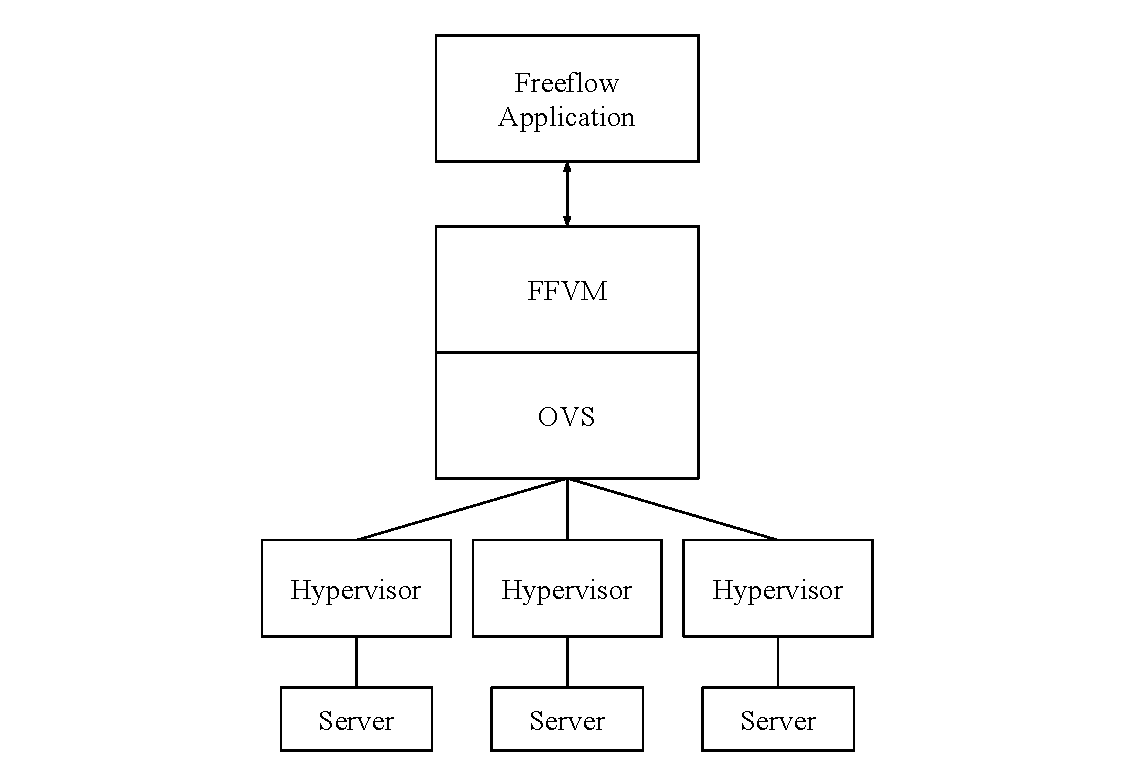
\includegraphics[scale=0.5]{ff_ovs_arch}
% \caption{Freeflow running ontop of OVS.}
% \label{ff_ovs_arch}
% \end{figure}